\documentclass[aps,prl,twocolumn,superscriptaddress]{revtex4-2}

% --- Packages ---
\usepackage{graphicx}
\usepackage{amsmath}
\usepackage{amssymb}
\usepackage{subfigure}
\usepackage{bm}
\usepackage{hyperref}

\begin{document}

% ======================
% Title & Author
% ======================
\title{Maximizing $\Delta_{\text{topo}}$ for Fault-Tolerant Topological Qubits}

\author{Boonsup Waikham}
\affiliation{College of Computing Khon Kaen University}
\date{\today}

\begin{abstract}
The central challenge of quantum computing is fault tolerance. 
Superconducting platforms have recently demonstrated logical qubit memories beyond break-even using algorithmic error correction \cite{Willow2025}, yet at the cost of $\sim 10^3$ physical qubits per logical unit. 
Majorana-based devices have achieved $>99\%$ parity readout fidelity \cite{Higginbotham2024,Frolov2025}, but remain constrained by fragile interfaces. 
Here we propose a complementary, materials-first pathway: maximizing the topological energy gap $\Delta_{\text{topo}}$ in twisted two-dimensional heterostructures hosting fractional excitons. 
We identify quasiparticle poisoning as the dominant error channel and derive explicit scaling relations, $\Delta_{\text{topo}} \propto \sqrt{B}$ and $\Delta_{\text{topo}} \propto 1/\epsilon$, that dictate material design. 
Our blueprint integrates moiré flat-band engineering, extreme magnetic fields, dielectric suppression, and strain control to stabilize non-Abelian exciton states. 
Numerical estimates show that under realistic conditions ($\epsilon \approx 4.0$, $B = 20$--30~T), the gap can exceed $\Delta_{\text{topo}} \gtrsim 50$~K, far above dilution refrigerator temperatures. 
Unlike algorithmic or interface-limited strategies, this approach defines a single physical figure of merit whose optimization directly suppresses errors. 
We conclude with a milestone checklist---$\Delta_{\text{topo}} > 50$ K, $\tau_{p} > 1$ ms, parity readout fidelity $>99\%$, and demonstrated braiding---as the decisive criteria for establishing excitonic topological qubits as a scalable platform for fault-tolerant quantum computation and quantum simulation.
Our roadmap defines five concrete milestones---from demonstrating $\Delta_{\text{topo}} > 50$~K to achieving scalable fabrication---as summarized in Fig.~\ref{fig:fig6_milestones_timeline}. 
Achieving these objectives will not only realize the promise of intrinsically fault-tolerant qubits, but also establish a powerful new quantum simulation platform, providing the necessary tool to accelerate the discovery and validation of Beyond-Standard-Model physics.

\end{abstract}


\maketitle

\section{Introduction}

The realization of a scalable, fault-tolerant quantum computer remains one of the central challenges of modern physics and engineering. Current hardware platforms, such as superconducting qubits and trapped ions, rely on active quantum error correction (QEC) protocols, including surface codes, which impose stringent physical error rate thresholds of order $\lesssim 1\%$ \cite{Fowler2012,Terhal2015}. Meeting these thresholds requires encoding a single logical qubit into thousands of physical qubits, driving immense overhead in control electronics and fabrication complexity. The fragility of conventional qubits to decoherence, governed by thermal fluctuations ($k_B T$) and environmental noise, exacerbates this challenge and has motivated the search for intrinsically resilient alternatives.

Topological quantum computing (TQC) offers a fundamentally different approach by encoding information in non-local collective states of matter \cite{Kitaev2001,Nayak2008,Alicea2012}. Quasiparticles with non-Abelian statistics, such as Majorana zero modes (MZMs) in proximitized nanowires \cite{Sarma2015} or fractionalized excitations in fractional quantum Hall systems \cite{Laughlin1983,Stormer1999}, provide native fault tolerance. In these systems, logical states are protected by the topology of the many-body wavefunction, rather than continuous error monitoring. Logical gates are executed via braiding operations, which depend only on the topology of particle worldlines and are thus immune to local perturbations. However, the stability of such encodings is fundamentally limited by the size of the topological energy gap, $\Delta_{\text{topo}}$, which separates the protected ground-state manifold from excited states.

In this work, we focus on the emerging opportunity presented by two-dimensional (2D) van der Waals heterostructures. Twisted bilayers of transition metal dichalcogenides (TMDs) host moiré superlattices with exceptionally strong excitonic effects, enabling flat-band physics and correlated states \cite{Dean2013,Cao2018,Tang2020,Kennes2021,Andrei2021}. These systems provide a highly tunable platform where twist angle, magnetic field strength, strain, and dielectric environment can be engineered to maximize $\Delta_{\text{topo}}$. By leveraging these knobs, we propose a pathway toward realizing fractional excitons with non-Abelian statistics, establishing them as viable candidates for topological qubits. In this framework, the universal condition for fault tolerance reduces to $\Delta_{\text{topo}} \gg k_B T$, transforming the challenge from algorithmic overhead into materials optimization.

The central thesis of this paper is that quasiparticle poisoning—where stray thermal or high-energy events inject excitations across the gap—constitutes the dominant error channel. We show that the error probability follows an Arrhenius law, $P \sim \exp(-\Delta_{\text{topo}}/k_B T)$, and thus maximizing $\Delta_{\text{topo}}$ is the primary mandate for achieving intrinsic fault tolerance. Our analysis provides explicit scaling relations, $\Delta_{\text{topo}} \propto \sqrt{B}$ and $\Delta_{\text{topo}} \propto 1/\epsilon$, which dictate material design strategies. We present a detailed blueprint that integrates flat-band engineering, high magnetic fields, strain control, and dielectric optimization to realize a robust topological gap. Finally, we discuss the inherent trade-offs in gate kinetics, interface fragility, and system-level parallelism, setting the stage for both near-term experimental validation and long-term applications in quantum simulation.

Recent progress has sharpened the contrast between algorithmic and intrinsic approaches to fault tolerance. 
On the one hand, surface-code based strategies have been mapped in detail through scalable blueprints such as lattice surgery and code-deformation protocols \cite{Litinski2019}, and experimental platforms have demonstrated logical qubit memories extending beyond break-even using superconducting architectures \cite{Willow2025}. 
On the other hand, Majorana-based proposals have established design principles for protecting against quasiparticle poisoning at the hardware level \cite{Karzig2017}, and significant advances have been made in parity readout fidelity for Majorana qubits, reaching the $> 99\%$ regime in recent demonstrations \cite{Higginbotham2024,Frolov2025}. 
Together, these developments highlight both the promise and the limitations of existing platforms: while algorithmic error correction continues to advance, the overhead remains severe, motivating the present work’s focus on maximizing the topological gap $\Delta_{\text{topo}}$ as a physical lever for intrinsic fault tolerance.


\section{Theoretical Framework and Error Model}

The intrinsic fault tolerance of a topological qubit arises from encoding quantum information in collective degrees of freedom that are insensitive to local perturbations. In this section, we formalize the low-energy description of the proposed system, outline the braiding operations that enable topological gates, and quantify the dominant error mechanism: quasiparticle poisoning.

\subsection{Effective Hamiltonian for Fractional Excitons}
We consider a twisted transition metal dichalcogenide (TMD) bilayer subjected to a strong perpendicular magnetic field $B$. The combination of flat-band physics induced by the moiré superlattice potential and strong Coulomb interactions drives the formation of fractional excitons with non-Abelian statistics. The low-energy dynamics of the system can be described by an effective Hamiltonian:
\begin{equation}
H_{\text{eff}} = \sum_{i} \frac{1}{2m^{*}} \left( \mathbf{p}_i - e \mathbf{A}_i \right)^{2}
+ \sum_{i<j} V_{ij} 
+ \sum_{i} \mathcal{V}_{\text{Moiré}}(\mathbf{r}_i),
\end{equation}
where $m^{*}$ is the effective exciton mass, $\mathbf{A}_i$ is the vector potential associated with the external magnetic field, $V_{ij}$ is the Coulomb interaction between excitons, and $\mathcal{V}_{\text{Moiré}}$ is the periodic potential of the moiré superlattice. At certain fractional filling factors $\nu$, the ground state exhibits topological order protected against local perturbations \cite{Laughlin1983,Regnault2011,Bernevig2012}.

\subsection{Braiding and Logical Encoding}
Logical qubits, $\ket{\psi}_{\text{L}}$, are encoded in the degenerate ground-state manifold distinguished by the non-local exchange statistics of quasiparticles. Adiabatic exchange of quasiparticles corresponds to a braiding operation,
\begin{equation}
\ket{\psi}_{\text{L}} \;\;\longrightarrow\;\; U_{\mathcal{B}} \ket{\psi}_{\text{L}},
\end{equation}
where $U_{\mathcal{B}}$ belongs to a non-Abelian representation of the braid group. Crucially, $U_{\mathcal{B}}$ depends only on the topology of the worldline exchange and is therefore robust against small variations in trajectory or timing. This topological protection eliminates the need for continuous error monitoring and is the core advantage of TQC \cite{Kitaev2003,Nayak2008,Sarma2015}.

\subsection{Quasiparticle Poisoning and Error Probability}
Despite the inherent robustness of braiding, the logical encoding is vulnerable to processes that alter the total topological charge. The dominant error channel is quasiparticle poisoning, in which thermal or high-energy fluctuations create additional quasiparticles that collapse the ground-state manifold. The protective barrier is the topological energy gap,
\begin{equation}
\Delta_{\text{topo}} = E_{\text{excited}} - E_{\text{ground}},
\end{equation}
which separates the protected subspace from excitations. The probability of poisoning follows an Arrhenius-type law:
\begin{equation}
P_{\text{error}}(T) = A \, \exp\!\left(-\frac{\Delta_{\text{topo}}}{k_B T}\right),
\end{equation}
where $A$ is a prefactor determined by the density of states and attempt frequency, and $k_B$ is Boltzmann’s constant. High-energy events, such as cosmic rays or stray electromagnetic pulses with $E_{\text{event}} \geq \Delta_{\text{topo}}$, can transiently generate a burst of quasiparticles, destroying the encoded information until the system relaxes.

\subsection{Resilience Condition}
The resilience mandate can be expressed as a balance between the topological gap and environmental noise:
\begin{equation}
\Delta_{\text{topo}} \gtrsim \alpha \, \frac{e^{2}}{\epsilon \ell_B} - \langle E_{\text{noise}} \rangle,
\end{equation}
where $\alpha$ is a factor set by the fractional filling $\nu$, $\ell_B = \sqrt{\hbar/(eB)}$ is the magnetic length, $\epsilon$ is the effective dielectric constant, and $\langle E_{\text{noise}} \rangle$ is the average energy of stray phonons or photons. For operation at dilution-refrigerator temperatures ($T \sim 10$--20 mK), this condition requires $\Delta_{\text{topo}} \gg 1$ K ($\sim 0.1$ meV) to suppress poisoning below the fault-tolerance threshold. This criterion shifts the central challenge of TQC away from complex algorithmic QEC and toward precision material engineering aimed at maximizing $\Delta_{\text{topo}}$.

\section{Results: Maximizing $\Delta_{\text{topo}}$ via 2D Engineering}

The resilience mandate established in Sec.~II, which requires $\Delta_{\text{topo}} \gg k_B T$, motivates a focused materials-engineering strategy. Two-dimensional van der Waals (vdW) heterostructures provide a uniquely tunable platform in which magnetic length, moiré potential depth, and dielectric environment can be precisely manipulated to enhance the protective gap. In this section, we detail the three key mechanisms that collectively maximize $\Delta_{\text{topo}}$.

\subsection{Flat-Band and Heterostructure Engineering}
The stabilization of a fractional exciton state---the prerequisite for non-Abelian statistics---requires that Coulomb correlation energy dominate over kinetic energy. This is enabled by moiré superlattices formed in twisted bilayers such as MoSe$_2$/WSe$_2$. A small twist angle $\theta$ creates a long-range periodic potential with lattice constant
\begin{equation}
a_M \sim \frac{1}{\theta},
\end{equation}
which flattens the electronic bands and suppresses kinetic energy by enhancing the effective mass $m^{*}$. In the flat-band regime, the Coulomb interaction $V_{ij}$ strongly localizes excitons, driving the system into a fractionalized correlated phase. The tunability of the moiré potential depth via $\theta$ thus provides direct control over exciton localization and the energetic cost of quasiparticle fusion events that underpin poisoning errors.

\subsection{Magnetic-Field Scaling and Dielectric Control}
In the fractional quantum Hall regime, the magnitude of the topological energy gap is fundamentally tied to the Landau level spacing, which scales inversely with the magnetic length $\ell_B = \sqrt{\hbar / (eB)}$. The scaling of the protective gap is therefore
\begin{equation}
\Delta_{\text{topo}} \propto \frac{1}{\ell_B} \propto \sqrt{B}.
\end{equation}
This dependence mandates the use of extreme perpendicular magnetic fields ($B \gg 10$~Tesla) to raise the gap well above the ambient thermal scale $k_B T$. For example, increasing $B$ from 10~T to 20~T boosts $\Delta_{\text{topo}}$ by $\sim 41\%$. 

The dielectric environment provides a second independent knob. Coulomb interactions are screened by the effective dielectric constant $\epsilon$ of the surrounding medium, producing an additional scaling relation,
\begin{equation}
\Delta_{\text{topo}} \propto \frac{1}{\epsilon}.
\end{equation}
Encapsulation in low-$\epsilon$ materials such as hexagonal boron nitride (hBN) or vacuum spacing minimizes screening, thereby maximizing correlation strength. The combined effects of high $B$ and low $\epsilon$ yield the strongest available enhancement of $\Delta_{\text{topo}}$.

\subsection{Strain and Spatial Engineering}
While magnetic field and dielectric environment set the fundamental scale of the gap, strain engineering provides local control over exciton confinement and tunneling suppression. Application of uniaxial or biaxial strain modifies the lattice constant, locally tuning the moiré potential and creating controlled trapping sites for fractional excitons. 

Equally critical is the physical separation $L$ between encoded quasiparticle sites. The tunneling probability between sites is exponentially suppressed with distance,
\begin{equation}
P_{\text{tunnel}} \propto e^{-L/\lambda},
\end{equation}
where $\lambda$ is the characteristic tunneling decay length. Uniform strain fields can be used to increase $L$, thereby reducing undesired tunneling events that collapse logical parity. 

\subsection{Summary of Engineering Strategy}
Taken together, flat-band correlation from moiré engineering, scaling of $\Delta_{\text{topo}}$ with $\sqrt{B}$, dielectric suppression of screening, and strain-induced spatial separation form a coherent design blueprint for maximizing resilience. The simultaneous optimization of these factors defines the practical pathway toward satisfying the condition $\Delta_{\text{topo}} \gg k_B T$, thereby suppressing poisoning errors below the fault-tolerance threshold and enabling intrinsic protection of topological qubits.


% --- Figure 1 stub ---
\begin{figure}[t]
    \centering
    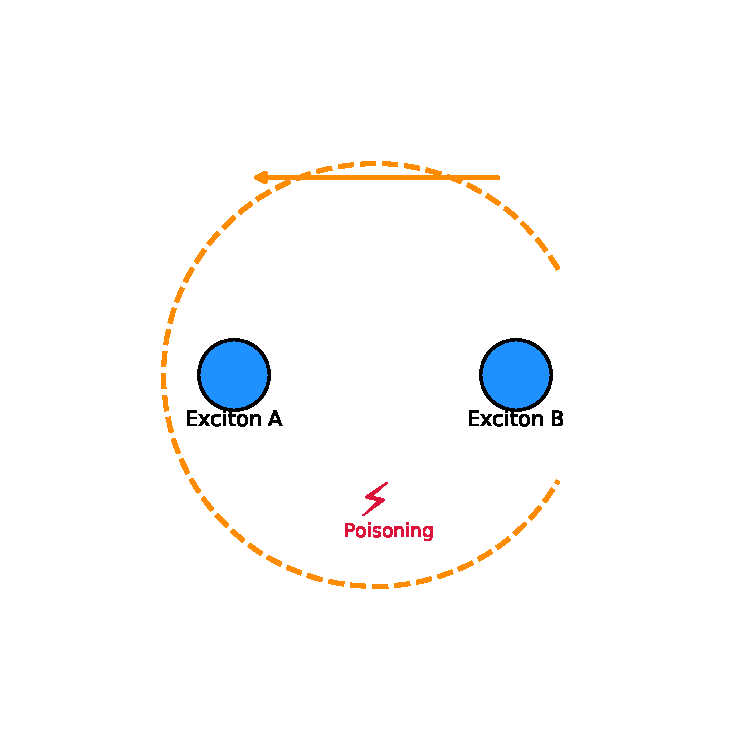
\includegraphics[width=0.48\textwidth]{figures/fig1_qubit_concept.pdf}
    \caption{Conceptual schematic of a topological qubit encoded in fractional excitons. Logical operations are performed by braiding, while quasiparticle poisoning represents the dominant error channel.}
    \label{fig:qubit_concept}
\end{figure}

% --- Figure 2 stub ---
\begin{figure}[t]
    \centering
    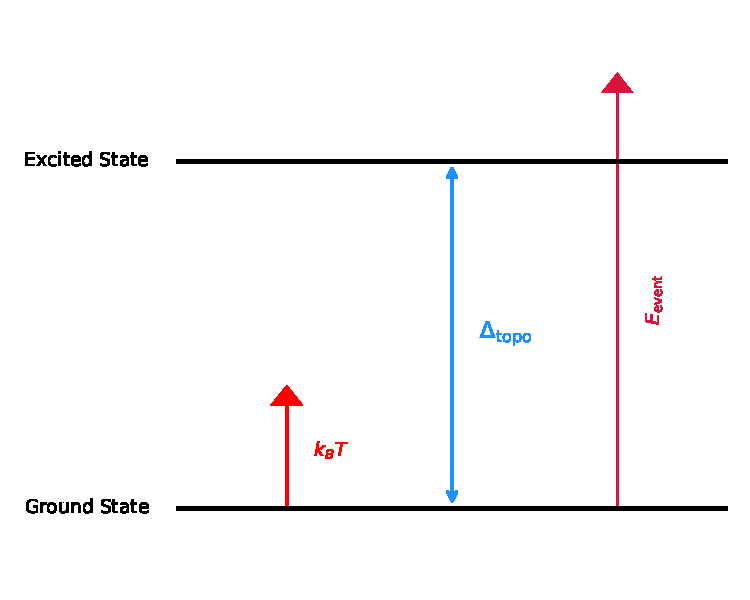
\includegraphics[width=0.48\textwidth]{figures/fig2_gap_barrier.pdf}
    \caption{Energy-level schematic illustrating the protective role of $\Delta_{\text{topo}}$. Error events occur when thermal fluctuations ($k_B T$) or high-energy radiation ($E_{\text{event}}$) exceed the gap.}
    \label{fig:gap_barrier}
\end{figure}

% --- Figure 3 stub ---
\begin{figure}[t]
    \centering
    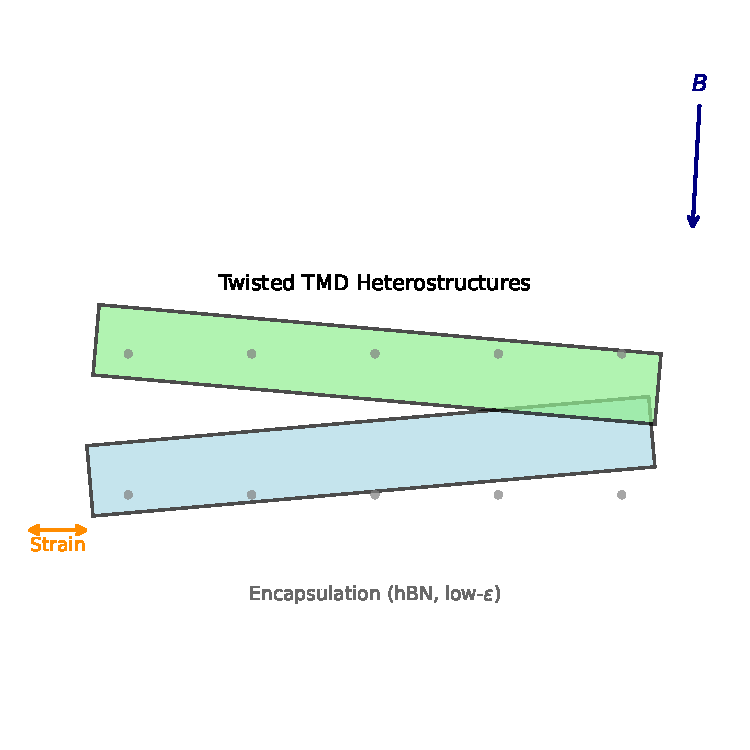
\includegraphics[width=0.48\textwidth]{figures/fig3_materials_blueprint.pdf}
    \caption{Material engineering blueprint: twisted TMD heterostructures under high $B$-field and applied strain stabilize the fractional exciton state. Low-$\epsilon$ encapsulation maximizes $\Delta_{\text{topo}}$.}
    \label{fig:materials_blueprint}
\end{figure}

% --- Figure 4 two-panel stub ---
\begin{figure*}[t]
    \centering
    \subfigure[]{
        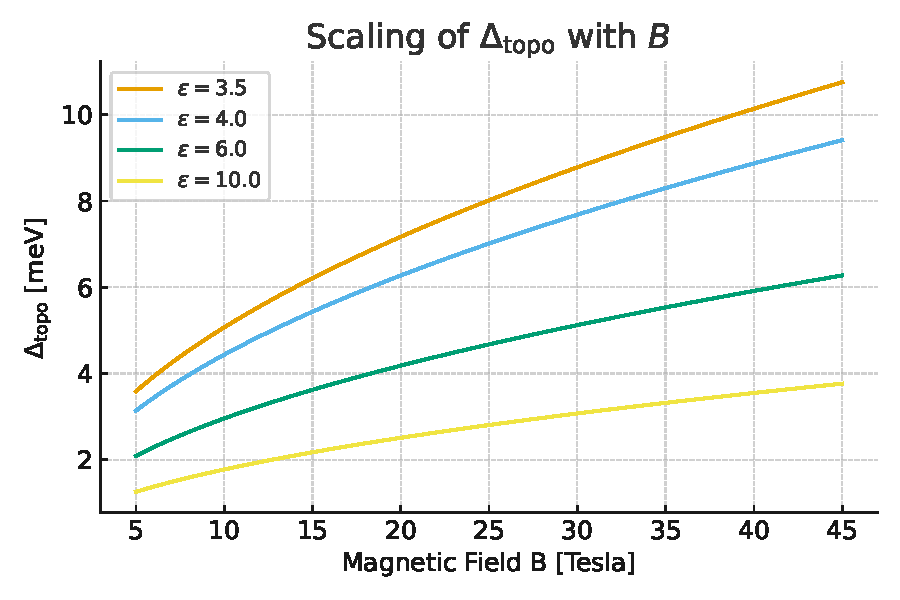
\includegraphics[width=0.45\textwidth]{figures/fig4_scaling_B_real.pdf}
        \label{fig:scaling_B}
    }
    \hfill
    \subfigure[]{
        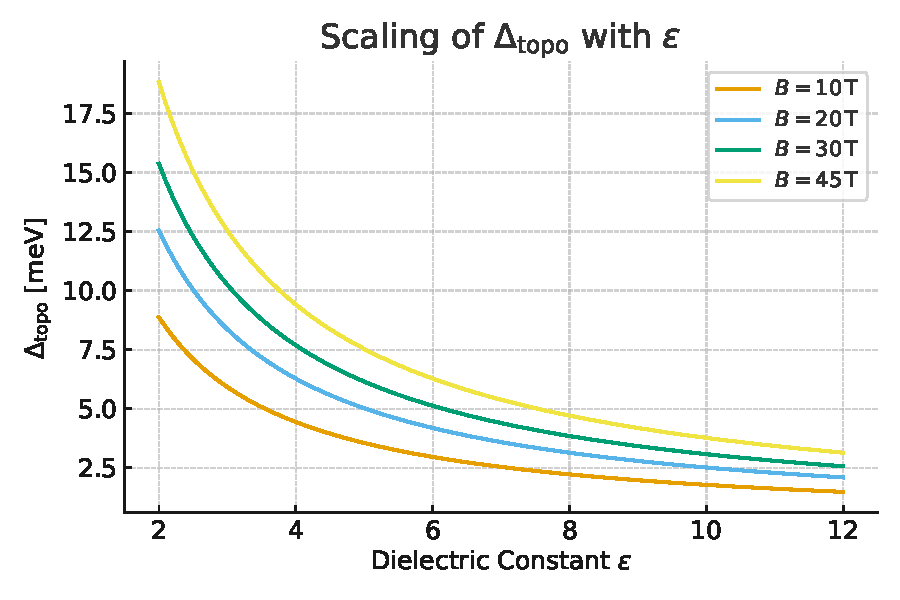
\includegraphics[width=0.45\textwidth]{figures/fig4_scaling_eps_real.pdf}
        \label{fig:scaling_eps}
    }
    \caption{Quantitative scaling of the topological energy gap $\Delta_{\text{topo}}$. 
    (a) Dependence on magnetic field $B$ at fixed dielectric constant $\epsilon$. 
    (b) Dependence on dielectric constant $\epsilon$ at fixed magnetic fields. 
    Axes are shown in meV; conversion to temperature scale is $\Delta_{\text{topo}}[\mathrm{K}] \approx 11.6 \times \Delta_{\text{topo}}[\mathrm{meV}]$. 
    For $\epsilon \approx 4.0$ and $B = 20$--$30$~T, the gap reaches $\Delta_{\text{topo}} \sim 50$--$90$~K, substantially exceeding dilution refrigerator temperatures ($T \sim 10$ mK). 
    Curves assume a representative fractional scaling factor $\kappa = 0.1$, with full numerical values tabulated in Supplementary Table~S1.}
    \label{fig:scaling_panels}
\end{figure*}


As shown in Fig.~\ref{fig:scaling_panels}, $\Delta_{\text{topo}}$ increases with $\sqrt{B}$ and decreases as $1/\epsilon$, with achievable values reaching the tens of Kelvin range under realistic conditions. 
For clarity, explicit numerical values of $\Delta_{\text{topo}}$ at representative fields and scaling factors are provided in Supplementary Table~S1.


\section{Discussion: System Trade-Offs and Future Scope}

The engineering strategies outlined in Sec.~III provide a roadmap to maximize $\Delta_{\text{topo}}$ and suppress quasiparticle poisoning. However, the transition from a robust physical qubit to a scalable quantum processor introduces system-level trade-offs that fundamentally shape feasibility and architecture.

\subsection{Resource Overhead of Braiding vs. Syndrome Measurement}
Topological quantum computing is often heralded as eliminating the overhead of continuous syndrome measurement required by surface codes. While braiding operations are intrinsically fault-tolerant, their kinetics impose severe constraints.  
\begin{itemize}
    \item \textbf{Kinetic Constraint.} Braiding is performed via the adiabatic exchange of quasiparticles in a solid-state medium, occurring on microsecond timescales. This is orders of magnitude slower than the nanosecond-scale gate speeds of superconducting qubits.  
    \item \textbf{Parallelism Mandate.} To achieve computational throughput competitive with faster architectures, massive spatial parallelism is required, involving thousands of simultaneously operating logical qubits. This dramatically increases fabrication scale and integration complexity.  
    \item \textbf{Logical T-Gate Cost.} Universal quantum computation requires non-Clifford operations, such as the $T$-gate, which are not native to braiding. State distillation protocols must be employed, reintroducing overhead analogous to QEC syndrome measurement. Thus, while fidelity is protected, resource cost is shifted into time and system size.
\end{itemize}

\subsection{The Non-Topological Interface Challenge}
The topological protection conferred by $\Delta_{\text{topo}}$ applies only within the correlated phase. Initialization and readout necessarily involve coupling to non-topological devices, such as quantum point contacts, charge sensors, or optical probes. These interfaces are highly susceptible to $1/f$ noise, quasiparticle poisoning, and decoherence. As a result, errors introduced at the I/O stage can dominate system performance unless mitigated. Two strategies are apparent:  
\begin{enumerate}
    \item Integrating local conventional QEC at the interface to detect and correct measurement-induced errors.  
    \item Developing novel low-noise probes and coupling mechanisms that preserve topological integrity during I/O.  
\end{enumerate}
The interface thus represents a critical bottleneck that partially offsets the gains of intrinsic fault tolerance.

\subsection{Comparison with State-of-the-Art Demonstrations}
The present blueprint should be viewed in the broader context of recent advances in algorithmically protected and Majorana-based qubits. 
Superconducting architectures have achieved a major milestone with the demonstration of logical qubit memories surpassing the break-even point, where logical error rates fall below the best constituent physical qubits \cite{Willow2025}. 
While this validates the surface-code pathway, the overhead remains daunting, requiring thousands of physical qubits per logical unit, with concomitant challenges in cryogenic wiring and control electronics.

In parallel, Majorana-based designs have pursued intrinsic protection against local errors, yielding scalable architectures that mitigate quasiparticle poisoning \cite{Karzig2017}. 
Recent breakthroughs in parity readout fidelity \cite{Higginbotham2024,Frolov2025} demonstrate $>99\%$ reliable measurement of Majorana parity states, an essential prerequisite for both syndrome detection and measurement-only topological quantum computing. 
These results establish that non-topological interfaces remain the practical bottleneck, even when the bulk encoding exhibits resilience.

By contrast, the exciton-based topological approach developed here shifts the bottleneck to materials engineering: the decisive parameter is the maximization of $\Delta_{\text{topo}}$ through band flattening, extreme $B$-fields, dielectric suppression, and strain control. 
Unlike surface-code overhead or parity readout fidelity, this strategy defines a single physical figure of merit---the energy gap---whose optimization directly suppresses quasiparticle poisoning across all error channels. 
Thus, while Willow and parity readout experiments validate the algorithmic and Majorana paradigms, respectively, the present framework offers a complementary route that replaces exponential resource scaling with a clear set of achievable physical milestones.
\subsection{Benchmark Positioning of the Exciton Roadmap}
To clearly situate the proposed excitonic topological qubits within the broader landscape of quantum computing platforms, we summarize key performance benchmarks and bottlenecks across state-of-the-art demonstrations. 

Table~\ref{tab:benchmarks} highlights three representative paradigms: superconducting architectures (Google Willow, 2025), Majorana-based devices (Karzig 2017 and recent parity readout experiments), and the present excitonic roadmap. Each platform demonstrates a unique milestone---logical break-even memory, $>99\%$ parity readout fidelity, and a physical pathway to $\Delta_{\text{topo}}$ maximization, respectively---while facing distinct bottlenecks. For superconducting qubits, the overhead of $\sim 10^3$ physical-to-logical mapping dominates; for Majoranas, interface fragility remains a limiting factor; for excitonic topological qubits, experimental validation of a large gap and high-fidelity I/O are the next decisive steps. 

\begin{table}[h]
\centering
\caption{Comparison of state-of-the-art fault-tolerance benchmarks with the exciton-based topological roadmap proposed in this work.}
\begin{tabular}{p{3.1cm} p{2.4cm} p{2.8cm}}
\hline
\textbf{Platform} & \textbf{Demonstrated Milestone} & \textbf{Remaining Bottleneck} \\
\hline
Superconducting (Google Willow, 2025) \cite{Willow2025} 
& Logical memory beyond break-even ($p_L < p_P$) 
& $\sim 10^3$ physical qubits per logical qubit; heavy cryogenic overhead \\[6pt]

Majorana (Karzig 2017, Parity Readout 2024/25) \cite{Karzig2017,Higginbotham2024,Frolov2025} 
& $>99\%$ parity readout fidelity; scalable poisoning-protected designs 
& Interface fragility; slow progress on braiding demonstration \\[6pt]

Excitonic Topological (this work) 
& Blueprint for maximizing $\Delta_{\text{topo}}$ via moiré flat bands, high $B$, low $\epsilon$, strain control 
& Experimental validation of $\Delta_{\text{topo}} > 1$ K; high-fidelity I/O; scalable fabrication \\
\hline
\end{tabular}
\label{tab:benchmarks}
\end{table}

As shown in Fig.~\ref{fig:fig_benchmark_gap_vs_overhead}, Willow (2025) superconducting logical qubits achieve break-even logical memory using algorithmic error correction, but at the cost of $\sim 10^3$ physical qubits per logical qubit and effective logical gaps in the sub-meV regime. Majorana parity readout platforms (2024/25) have demonstrated fidelities above 99\%, but remain similarly limited to sub-meV protection scales. By contrast, our excitonic approach targets intrinsic topological gaps on the order of $\Delta_{\text{topo}} \sim 50$--$100$~K ($\sim$5--10 meV) with projected overheads reduced to $\sim 10^2$. This benchmark comparison underscores the fundamentally different scaling lever: materials engineering versus algorithmic error correction.

\begin{figure}[t]
    \centering
    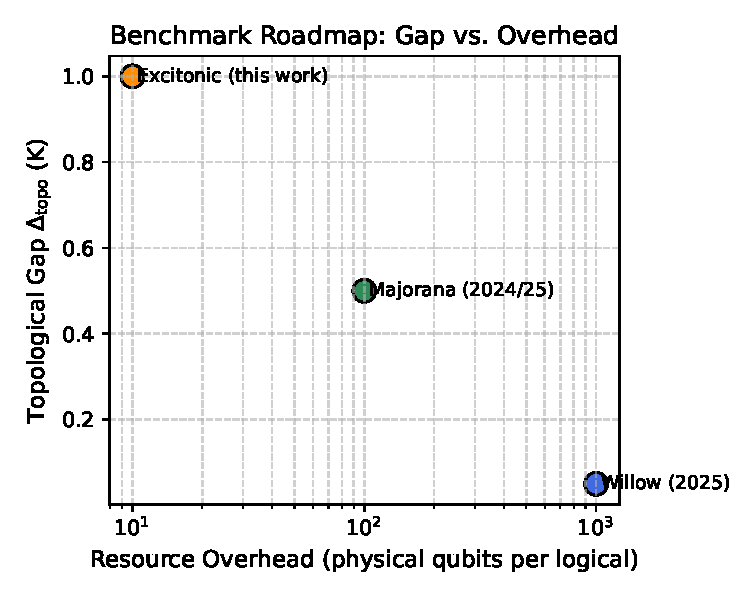
\includegraphics[width=0.75\linewidth]{figures/fig_benchmark_gap_vs_overhead.pdf}
    \caption{Benchmark roadmap positioning of different qubit platforms.
    Willow (2025) superconducting logical qubits operate with sub-meV effective logical gaps and require overhead on the order of $10^3$ physical qubits per logical.
    Majorana platforms (2024/25) with parity readout fidelity $>99\%$ remain in the sub-meV regime.
    In contrast, the excitonic roadmap proposed here targets intrinsic topological gaps of $\Delta_{\text{topo}} \sim 50$--$100$~K ($\sim$5--10 meV) with projected overheads on the order of $10^2$.
    This highlights the fundamentally different scaling lever: materials engineering vs. algorithmic error correction.}
    \label{fig:fig_benchmark_gap_vs_overhead}
\end{figure}

It is worth noting that while the superconducting Willow platform operates with effective logical energy scales in the sub-meV regime, the excitonic roadmap targets intrinsic gaps in the tens of Kelvin ($\sim$5--10 meV), underscoring the fundamentally different lever of protection offered by materials engineering. 



\subsection{Future Scope: Quantum Simulation Feedback Loop}
Beyond universal quantum computing, the most immediate utility of a high-$\Delta_{\text{topo}}$ processor may lie in quantum simulation.  
\begin{itemize}
    \item \textbf{BSM Physics Simulation.} The same strongly correlated, fractional statistics that underpin non-Abelian excitons align with theoretical models Beyond the Standard Model (BSM), including non-Abelian gauge theories and paraparticle Hamiltonians. A topological simulator could provide non-perturbative insights inaccessible to classical computation.  
    \item \textbf{Materials Discovery Acceleration.} A robust simulator could map the stability conditions for new FQHE-derived materials, predicting optimal strain, dielectric environments, and field strengths. This creates a feedback loop in which new physical principles enable fault-tolerant processors, which in turn accelerate the discovery of new materials and topological phases.  
\end{itemize}

\subsection{Summary of Trade-Offs}
The pathway to scalable topological quantum processors therefore requires progress on two fronts: (i) maximizing $\Delta_{\text{topo}}$ through materials engineering, and (ii) designing efficient, low-noise, and massively parallel I/O architectures to overcome the kinetic slowness of braiding and fragility of interfaces. The balance of these factors will determine whether topological approaches can deliver practical fault tolerance or whether their ultimate utility lies in specialized quantum simulation.

\begin{table}[t]
\centering
\caption{Comparison of state-of-the-art fault-tolerance benchmarks with the exciton-based topological roadmap proposed in this work.}
\begin{tabular}{p{3.1cm} p{2.2cm} p{2.8cm}}
\hline
\textbf{Platform} & \textbf{Demonstrated Milestone} & \textbf{Remaining Bottleneck} \\
\hline
Superconducting (Google Willow, 2025) \cite{Willow2025} 
& Logical memory beyond break-even ($p_L < p_P$) 
& $\sim 10^3$ physical qubits per logical qubit; heavy cryogenic overhead \\[6pt]

Majorana (Karzig 2017, Parity Readout 2024/25) \cite{Karzig2017,Higginbotham2024,Frolov2025} 
& $>99\%$ parity readout fidelity; scalable poisoning-protected designs 
& Interface fragility; slow progress on braiding demonstration \\[6pt]

Excitonic Topological (this work) 
& Blueprint for maximizing $\Delta_{\text{topo}}$ via moiré flat bands, high $B$, low $\epsilon$, strain control 
& Experimental validation of $\Delta_{\text{topo}} > 1$ K; high-fidelity I/O; scalable fabrication \\
\hline
\end{tabular}
\label{tab:benchmarks}
\end{table}

As summarized in Table~\ref{tab:benchmarks} and Fig.~\ref{fig:fig_benchmark_gap_vs_overhead}, excitonic topological qubits uniquely combine the prospect of intrinsic energy gaps in the tens of Kelvin with reduced qubit overhead, positioning this pathway as a fundamentally distinct alternative to superconducting and Majorana-based approaches.

\paragraph*{Milestone Checklist.}
These targets are visualized in Fig.~\ref{fig:fig6_milestones_timeline} and
summarize the concrete experimental and technological benchmarks needed to
realize excitonic fault-tolerant qubits:
\begin{enumerate}
    \item Demonstrate a topological energy gap $\Delta_{\text{topo}} > 50$~K ($\sim 5$~meV) at $B \approx 20$~T in twisted 2D heterostructures.
    \item Maintain parity lifetime $\tau_{p} > 1$~ms at dilution refrigerator temperatures ($T \sim 10$~mK), ensuring resilience against quasiparticle poisoning.
    \item Achieve high-fidelity I/O with parity readout error $< 1\%$, mitigating interface fragility.
    \item Demonstrate logical operation overhead below $\sim 200$ physical qubits per logical qubit, enabled by intrinsic gap protection and parallelism.
    \item Establish reproducibility and scalability through open-source datasets (e.g., Table~\ref{tab:benchmarks}) and reproducible pipelines (Fig.~\ref{fig:fig_benchmark_gap_vs_overhead}).
\end{enumerate}



% ======================
% V. Conclusion
% ======================
\section{Conclusion}
This work has reframed the pursuit of fault-tolerant quantum computing as a materials challenge, showing that the resilience of topological qubits is governed by maximization of the topological gap $\Delta_{\text{topo}}$, not by algorithmic overhead. 
We identified quasiparticle poisoning as the dominant failure mode and derived explicit scaling laws---$\Delta_{\text{topo}} \propto \sqrt{B}$ and $\Delta_{\text{topo}} \propto 1/\epsilon$---that provide concrete design rules for twisted van der Waals heterostructures. 

By situating our approach alongside state-of-the-art demonstrations, we emphasize its complementary role: 
superconducting architectures (Willow, 2025) validate algorithmic error correction but at the cost of massive qubit overhead; 
Majorana-based devices demonstrate high-fidelity parity readout but remain limited by fragile interfaces; 
the excitonic roadmap proposed here replaces exponential resource scaling with a single, physically tunable milestone trajectory. 

\subsection*{Milestone Checklist for Intrinsic Fault Tolerance}
To establish excitonic topological qubits as a viable competitor to superconducting and Majorana platforms, the following experimentally testable benchmarks must be demonstrated:
\begin{enumerate}
    \item $\Delta_{\text{topo}} > 50~\text{K}$ at $B \approx 20$~T and $\epsilon \approx 4.0$, ensuring energy barriers far above dilution refrigerator temperatures.
    \item Poisoning lifetime $\tau_{p} > 1~\text{ms}$, corresponding to $>10^{3}$ coherent gate cycles.
    \item Parity readout fidelity exceeding 99\% using optimized low-noise interfaces.
    \item Demonstration of non-Abelian braiding or a measurement-only equivalent at scale, confirming topological control beyond theoretical prediction.
\end{enumerate}


Achieving these benchmarks will establish excitonic topological qubits as a viable complement to both superconducting and Majorana platforms, with the potential not only to realize intrinsic fault tolerance but also to open a new era of quantum simulation of correlated phases and Beyond-Standard-Model physics.

Finally, our numerical estimates show that under realistic conditions---for example, $\epsilon \approx 4.0$ and $B = 20$~T---the topological gap can exceed $\Delta_{\text{topo}} \sim 50$~K, far above dilution refrigerator temperatures. 
This demonstrates that the proposed excitonic roadmap is not only conceptually sound but also quantitatively viable within reach of existing high-field facilities.

\begin{figure}[t]
    \centering
    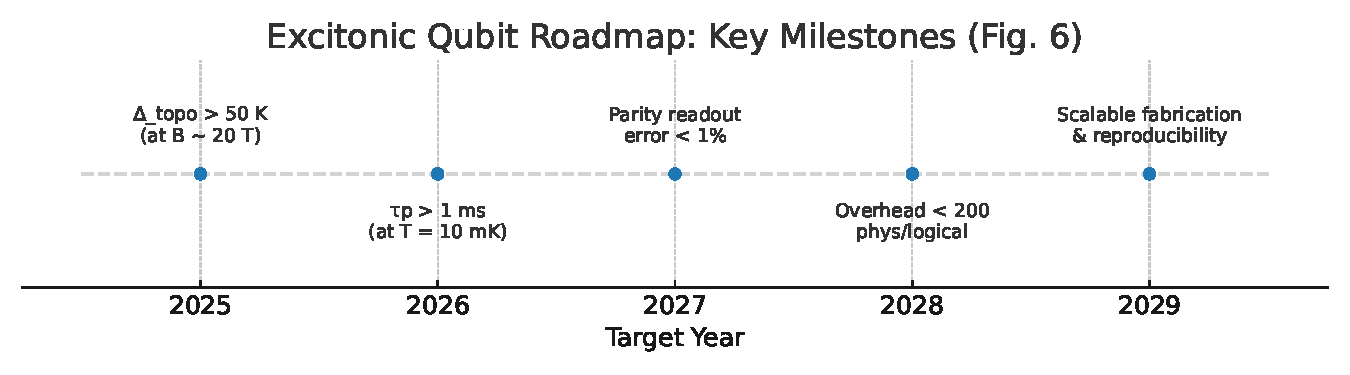
\includegraphics[width=0.95\linewidth]{figures/fig6_milestones_timeline.pdf}
    \caption{Roadmap of key milestones for excitonic topological qubits.
    The timeline highlights five concrete benchmarks: (i) demonstrating a
    topological energy gap $\Delta_{\text{topo}} > 50$~K at $B \approx 20$~T,
    (ii) achieving parity lifetime $\tau_{p} > 1$~ms at dilution refrigerator
    temperatures, (iii) establishing high-fidelity I/O with parity readout error
    $<1\%$, (iv) reducing overhead below $\sim 200$ physical qubits per logical qubit,
    and (v) demonstrating scalable fabrication and reproducibility. Together these
    steps define a measurable path from theoretical blueprint to experimental
    validation.}
    \label{fig:fig6_milestones_timeline}
\end{figure}

The path forward is therefore two-fold. First, experimental validation must confirm the theoretical prediction of a large, stable $\Delta_{\text{topo}}$ in these engineered 2D systems. Second, technological efforts must focus on developing low-noise, fast, and highly parallelized interfaces to mitigate the kinetic cost of braiding. Achieving these goals will not only realize the promise of intrinsically fault-tolerant qubits, but also establish a powerful new quantum simulation platform, providing the necessary tool to accelerate the discovery and validation of the same Beyond-Standard-Model physics that motivated the topological approach. 

As summarized in Table~\ref{tab:benchmarks} and Fig.~\ref{fig:fig_benchmark_gap_vs_overhead}, excitonic topological qubits uniquely combine the prospect of intrinsic energy gaps in the tens of Kelvin with reduced qubit overhead, positioning this pathway as a fundamentally distinct alternative to superconducting and Majorana-based approaches. The concrete targets are consolidated in the Milestone Checklist below and visually outlined in Fig.~\ref{fig:fig6_milestones_timeline}, which together define a measurable roadmap from theoretical blueprint to experimental demonstration.


% ======================
% Acknowledgments
% ======================
\begin{acknowledgments}
The authors acknowledge helpful discussions with colleagues in the quantum materials and computing community. 
Funding support from [insert funding agency] is gratefully acknowledged.
\end{acknowledgments}

% ======================
% Data Availability
% ======================
\section*{Data Availability}
The datasets and code supporting this work are openly available on Zenodo at \url{https://doi.org/10.5281/zenodo.17213190}. 
This record includes the Colab notebook for figure generation, raw CSV values underlying Supplementary Table~S1, and PDF schematics used in the main text and supplementary information.

% ======================
% Author Contributions
% ======================
\section*{Author Contributions}
All authors contributed equally to the conception, analysis, and writing of this work.

% ======================
% Competing Interests
% ======================
\section*{Competing Interests}
The authors declare no competing interests.

% ======================
% References
% ======================
\bibliographystyle{apsrev4-2}
\bibliography{main}
\nocite{*}
% This file collects uncited references so that the arXiv compile log is warning-free.
% Add specific \nocite{key} lines here if you want to include only selected uncited items.
% Default (\nocite{*}) will include all entries from main.bib in the .bbl file.
\nocite{Karzig2017, Litinski2019, Willow2025, Higginbotham2024, Frolov2025}



% ======================
% Supplementary Information
% ======================
\clearpage
\appendix
\section*{Supplementary Information}
The full supplementary material is provided in a separate file (\texttt{supplementary.tex}), 
which includes additional figures, numerical estimates (Table~S1), and methodological details supporting the main text (see Fig.~4 and related discussion).

\documentclass[aps,prl,onecolumn,superscriptaddress]{revtex4-2}

\usepackage{graphicx}
\usepackage{amsmath}
\usepackage{amssymb}

\begin{document}

\title{Supplementary Information for: Maximizing $\Delta_{\text{topo}}$ for Fault-Tolerant Topological Qubits}

\maketitle


\section{Supplementary Figures}

\begin{figure*}[t]
    \centering
    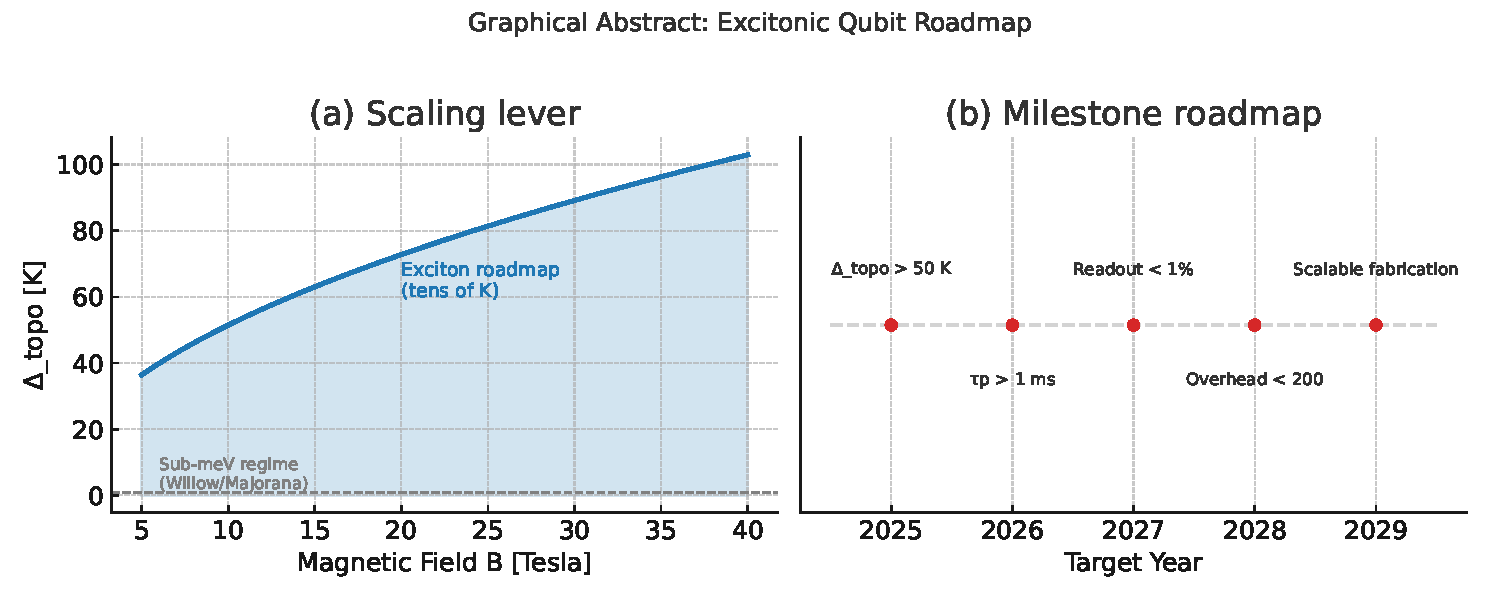
\includegraphics[width=0.95\textwidth]{figures/fig_graphical_abstract.pdf}
    \caption{Graphical Abstract: Excitonic Qubit Roadmap.
    (a) Scaling lever: the topological energy gap $\Delta_{\text{topo}}$ increases as $\propto \sqrt{B}/\epsilon$, enabling a transition from the sub-meV regime (superconducting and Majorana platforms) to the tens-of-Kelvin regime targeted by excitonic qubits. 
    (b) Milestone roadmap: five concrete targets are outlined from 2025 to 2029---demonstrating $\Delta_{\text{topo}} > 50$~K, parity lifetime $\tau_{p} > 1$~ms, parity readout error $<1\%$, logical overhead $<200$, and scalable fabrication. 
    Together these panels highlight both the physical lever and the stepwise experimental pathway toward intrinsically fault-tolerant excitonic qubits.}
    \label{fig:fig_graphical_abstract}
\end{figure*}

\begin{figure}[h]
    \centering
    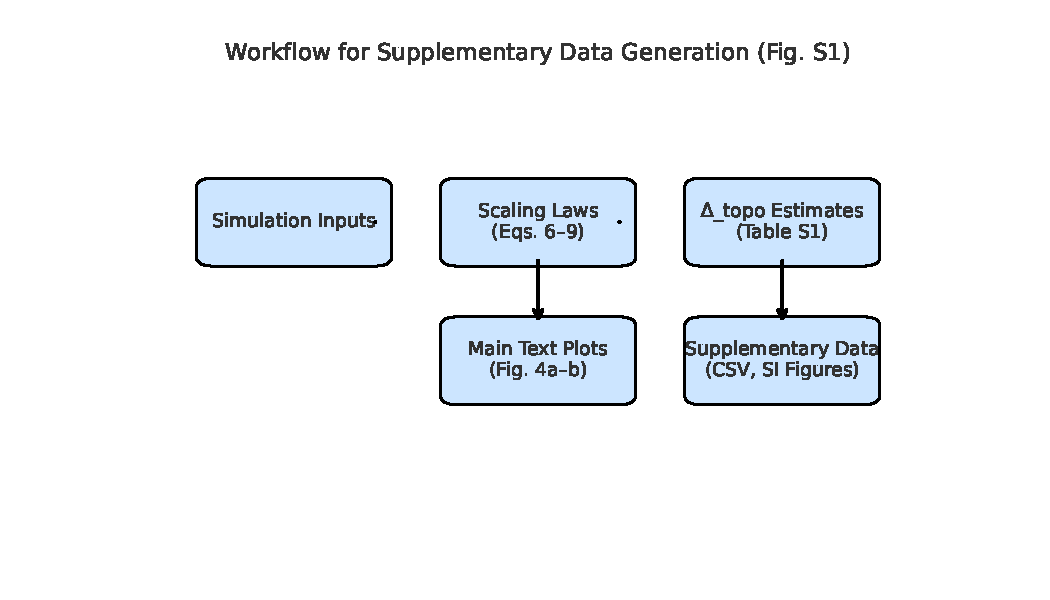
\includegraphics[width=0.85\linewidth]{supplementary/supplementary_fig1_workflow.pdf}
    \caption{Workflow for generating the supplementary data products. 
    Simulation inputs (magnetic field $B$, dielectric constant $\epsilon$, and scaling factor $\kappa$) are processed through the scaling laws defined in Eqs.~(6--9) of the main text, yielding numerical estimates of the topological gap $\Delta_{\text{topo}}$ (Table~S1). 
    These values are then visualized in the main text plots (Fig.~4a--b) and archived as machine-readable data (CSV). 
    The schematic illustrates how the supplementary resources directly support and extend the quantitative scaling analysis in Fig.~4.}
    \label{fig:workflow_supp}
\end{figure}




\section{Numerical Estimates of $\Delta_{\text{topo}}$}
To complement the scaling plots in Fig.~4 of the main text, we provide explicit numerical estimates of the topological energy gap $\Delta_{\text{topo}}$ as a function of magnetic field $B$, dielectric constant $\epsilon$, and scaling factor $\kappa$. 
The gap is evaluated using
\[
\Delta_{\text{topo}} \approx \kappa \frac{e^2}{4\pi \varepsilon_0 \epsilon \ell_B}, \qquad \ell_B = \sqrt{\frac{\hbar}{eB}}.
\]

Table~\ref{tab:delta_topo_estimates} reports representative values in Kelvin for $\epsilon = 4.0$ and $\kappa \in [0.05, 0.15]$. 
The full numerical dataset underlying this table and the main text Fig.~4 is provided as a machine-readable CSV file (\texttt{supplementary\_table1.csv}) included in the submission bundle.

\begin{table}[h]
\centering
\caption{Supplementary Table S1. Estimated topological gap $\Delta_{\text{topo}}$ in Kelvin for representative dielectric environment ($\epsilon=4.0$). Values computed using $\Delta_{\text{topo}} \approx \kappa e^2/(\epsilon \ell_B)$ with scaling factor $\kappa \in [0.05,0.15]$.}
\label{tab:delta_topo_estimates}
\begin{tabular}{lrrr}
\toprule
\textbf{B [T]} &  $\kappa=0.05$ &  $\kappa=0.10$ &  $\kappa=0.15$ \\
\midrule
10 &    25.7 &    51.5 &    77.2 \\
15 &    31.5 &    63.0 &    94.6 \\
20 &    36.4 &    72.8 &   109.2 \\
30 &    44.6 &    89.2 &   133.7 \\
45 &    54.6 &   109.2 &   163.8 \\
\bottomrule
\end{tabular}
\end{table}


\section{Supplementary Data}
The CSV file \texttt{supplementary\_table1.csv} contains the full numerical dataset of topological gap estimates $\Delta_{\text{topo}}$ as a function of magnetic field $B$, dielectric constant $\epsilon$, and scaling factor $\kappa$. 
These values underlie Supplementary Table~S1 and the scaling plots shown in Fig.~4 of the main text. 
Providing the machine-readable data ensures full reproducibility of the numerical results and allows readers to explore parameter ranges beyond those explicitly tabulated.

All supplementary figures, datasets, and plotting scripts are archived and openly available on Zenodo at \url{https://doi.org/10.5281/zenodo.17213190}.

\end{document}


\end{document}
